\documentclass{beamer}

\mode<presentation> {

%\usetheme{default}
%\usetheme{AnnArbor}
%\usetheme{Antibes}
%\usetheme{Bergen}
%\usetheme{Berkeley}
%\usetheme{Berlin}
%\usetheme{Boadilla}
%\usetheme{CambridgeUS}
%\usetheme{Copenhagen}
%\usetheme{Darmstadt}
%\usetheme{Dresden}
%\usetheme{Frankfurt}
%\usetheme{Goettingen}
%\usetheme{Hannover}
%\usetheme{Ilmenau}
%\usetheme{JuanLesPins}
%\usetheme{Luebeck}
\usetheme{Madrid}
%\usetheme{Malmoe}
%\usetheme{Marburg}
%\usetheme{Montpellier}
%\usetheme{PaloAlto}
%\usetheme{Pittsburgh}
%\usetheme{Rochester}
%\usetheme{Singapore}
%\usetheme{Szeged}
%\usetheme{Warsaw}


%\usecolortheme{albatross}
%\usecolortheme{beaver}
%\usecolortheme{beetle}
%\usecolortheme{crane}
%\usecolortheme{dolphin}
%\usecolortheme{dove}
%\usecolortheme{fly}
%\usecolortheme{lily}
%\usecolortheme{orchid}
%\usecolortheme{rose}
%\usecolortheme{seagull}
%\usecolortheme{seahorse}
%\usecolortheme{whale}
%\usecolortheme{wolverine}

%\setbeamertemplate{footline} % To remove the footer line in all slides uncomment this line
%\setbeamertemplate{footline}[page number] % To replace the footer line in all slides with a simple slide count uncomment this line

%\setbeamertemplate{navigation symbols}{} % To remove the navigation symbols from the bottom of all slides uncomment this line
}

\usepackage{graphicx} % Allows including images
\usepackage{booktabs} % Allows the use of \toprule, \midrule and \bottomrule in tables
\usepackage{amsfonts}
\usepackage{mathrsfs}
\usepackage{amsmath,amssymb,graphicx}
\usepackage{bm}  % for bold greek letters

%----------------------------------------------------------------------------------------
%	TITLE PAGE
%----------------------------------------------------------------------------------------

\title["2.5"]{2.5: Forecasting Stationary Time Series}

\author{Taylor} 
\institute[UVA] 
{
University of Virginia \\
\medskip
\textit{} 
}
\date{} 

\begin{document}
%----------------------------------------------------------------------------------------

\begin{frame}
\titlepage 
\end{frame}
%----------------------------------------------------------------------------------------

\begin{frame}
\frametitle{Motivation}

Goal of this section, assuming we know $\gamma$ and $\mu$, find a linear combination of $1, X_1, \ldots, X_n$ that does the ``best" job of forecasting $X_{n+h}$, for some $h\in \mathbb{Z}^+$.
\end{frame}

%----------------------------------------------------------------------------------------

\begin{frame}
\frametitle{Notation}

The best linear predictor is denoted $P_n X_{n+h}$. We need to figure out the the coefficients $a_0, a_1, \ldots, a_n$ that minimize the Mean Square Error (MSE)
\[
S(a_0, \ldots, a_n) = E[(X_{n+h} - \{a_0 + a_1X_n\cdots + a_nX_1 \} )^2].
\]
Clearly $S \ge 0$. To minimize we can take derivatives with respect to coefficients and set equal to $0$. 
\[
E[(X_{n+h} - \{a_0 + a_1X_n\cdots + a_nX_1 \} )] = 0
\]
and
\[
E[(X_{n+h} - \{a_0 + a_1X_n + \cdots + a_n X_1 \} ) X_{n+1-j} ] = 0, j=1,\ldots,n
\]


\end{frame}

%----------------------------------------------------------------------------------------


\begin{frame}
\frametitle{Motivation}

Re-arranging and keeping in mind that $j=1,\ldots,n$
\begin{align*}
E[(X_{n+h} - \{a_0 + a_1X_n\cdots + a_nX_1 \} )] &= 0 \\
E[(X_{n+h} - \{a_0 + a_1X_n + \cdots + a_n X_1 \} ) X_{n+1-j} ] &= 0
\end{align*}
becomes
\[
a_0 = \mu\left(1 - \sum_{i=1}^n a_i\right)
\]
\[
E[X_{n+h}X_{n+1-j}] =a_0\mu + \sum_{i=1}^na_i E[X_{n+1-i}X_{n+1-j} ] 
\]
or
\[
E[X_{n+h}X_{n+1-j}] - \mu^2 =a_0\mu + \sum_{i=1}^na_i E[X_{n+1-i}X_{n+1-j} ] -\mu^2
\]

\end{frame}

%----------------------------------------------------------------------------------------

\begin{frame}
\frametitle{Motivation}

Re-writing that last line
\[
E[X_{n+h}X_{n+1-j}] - \mu^2 = a_0\mu + \sum_{i=1}^na_i E[X_{n+1-i}X_{n+1-j} ] -\mu^2
\]
\begin{align*}
E[X_{n+h}X_{n+1-j}] - \mu^2 &= a_0\mu + \sum_{i=1}^na_i E[X_{n+1-i}X_{n+1-j} ] -\mu^2 \\
&=  \mu^2 \left(1 - \sum_{i=1}^n a_i\right) + \sum_{i=1}^na_i E[X_{n+1-i}X_{n+1-j} ] -\mu^2 \\
&=  - \mu^2 \sum_{i=1}^n a_i + \sum_{i=1}^na_i E[X_{n+1-i}X_{n+1-j} ] \\
&= \sum_{i=1}^n a_i \gamma(i-j)
\end{align*}

\end{frame}

%----------------------------------------------------------------------------------------
\begin{frame}
\frametitle{The prediction equations}

Writing everything with matrices and vectors we have 
\begin{block}{The Prediction Equations}
$P_n$ is determined by the $(a_0, a_1, \ldots, a_n)$ that satisify
\[
a_0 = \mu\left(1 - \sum_{i=1}^n a_i\right)
\]
and
\[
\Gamma_n \mathbf{a}_n = \gamma_n(h)
\]
where $\gamma_n(h) = (\gamma(h), \ldots, \gamma(h+n-1))'$ and $\Gamma_n = [\gamma(i-j)]_{i,j=1}^n$
\end{block}
\end{frame}

%----------------------------------------------------------------------------------------
\begin{frame}
\frametitle{The Best MSE}

Once we have $\mathbf{a}_n$ we can find the lowest possible MSE
\begin{align*}
E[(X_{n+h}-P_nX_{n+h})^2] &= \text{Var}[X_{n+h} - a_0 - a_1X_n\cdots - a_nX_1 ]\\
&= \text{Var}[X_{n+h} - a_1X_n\cdots - a_nX_1 ] \\
&= \text{Cov}(X_{n+h} - \sum_{i=1}^n a_i X_{n-i+1}, X_{n+h} - \sum_{i=1}^n a_i X_{n-i+1})\\
&= \gamma(0) - 2 \sum_{i=1}^na_i \gamma(h+i-1) + \sum_{i=1}^n \sum_{j=1}^n a_i a_j \gamma(j-i) \\
&= \gamma(0) - 2 \mathbf{a}_n'\gamma_n(h) + \mathbf{a}_n' \Gamma_n \mathbf{a}_n \\
&= \gamma(0) - 2 \mathbf{a}_n'\gamma_n(h) + \mathbf{a}_n'\gamma_n(h) \\
&= \gamma(0) -  \mathbf{a}_n'\gamma_n(h)
\end{align*}

\end{frame}


%----------------------------------------------------------------------------------------


\begin{frame}
\frametitle{Example}

Let's derive the $h$-step ahead prediction operator for a causal, mean-zero AR(1) model $X_t = \phi X_{t-1} + Z_t$.
\[
a_0 = \mu\left(1 - \sum_{i=1}^n a_i\right)
\]
and
\[
\Gamma_n \mathbf{a}_n = \gamma_n(h)
\]
becomes (after dividing both sides by $\gamma(0)$)
\begin{eqnarray}
\left[ \begin{array}{ccccc}
1 & \phi & \phi^2 & \cdots & \phi^{n-1} \\
\phi & 1 & \phi & \cdots & \phi^{n-2} \\
\vdots & \vdots & \vdots & \vdots & \vdots \\
\phi^{n-1} & \phi^{n-2} & \phi^{n-3} & \cdots & 1
\end{array}\right]
\left[\begin{array}{c}
a_1 \\
a_2 \\
\vdots \\
a_n
\end{array}\right]
=
\left[ \begin{array}{c}
\phi^h \\
\phi^{h+1} \\
\vdots \\
\phi^{h+n-1}
\end{array}\right]
\end{eqnarray}
solution: $\mathbf{a}_n = (\phi^h, 0, \ldots, 0)'$. What happens as you try to predict farther out?
\end{frame}

%----------------------------------------------------------------------------------------


\begin{frame}
\frametitle{Example}

What about if we include a mean? $X_t = \mu + \phi (X_{t-1} - \mu) + Z_t$ where the errors are white noise with variance $\sigma^2$. Now the intercept $a_0 \neq 0$.
\newline

We have this same set of equations again (same as last slide)
\[
\Gamma_n \mathbf{a}_n = \gamma_n(h) 
\]
but now we have this part ( because $\mu \neq 0$)
\[
a_0 = \mu\left(1 - \sum_{i=1}^n a_i\right) .
\]
So the solution is the same but now we have an extra $\alpha_0$ term.
\newline

% \begin{eqnarray}
% \left[ \begin{array}{ccccc}
% 1 & \phi & \phi^2 & \cdots & \phi^{n-1} \\
% \phi & 1 & \phi & \cdots & \phi^{n-2} \\
% \vdots & \vdots & \vdots & \vdots & \vdots \\
% \phi^{n-1} & \phi^{n-2} & \phi^{n-3} & \cdots & 1
% \end{array}\right]
% \left[\begin{array}{c}
% a_1 \\
% a_2 \\
% \vdots \\
% a_n
% \end{array}\right]
% =
% \left[ \begin{array}{c}
% \phi^h \\
% \phi^{h+1} \\
% \vdots \\
% \phi^{h+n-1}
% \end{array}\right]
% \end{eqnarray}
\end{frame}

%----------------------------------------------------------------------------------------


\begin{frame}
\frametitle{Properties of Prediction Operator}

\begin{block}{Properties of $P_n$}
\begin{itemize}
\item $P_nX_{n+h} = \mu + \sum_{i=1}^na_i(X_{n+1-i} - \mu)$
\item $E[(X_{n+h}-P_nX_{n+h})^2] = \gamma(0) -  \mathbf{a}_n'\gamma_n(h)$
\item $E(X_{n+h}-P_nX_{n+h}) = 0$
\item $E[(X_{n+h}-P_nX_{n+h})X_j] = 0$ for $j=1,\ldots,n$
\item $P_nX_{n+h}$ is unique.
\end{itemize}
\end{block}


\end{frame}

%----------------------------------------------------------------------------------------


\begin{frame}[fragile]
\frametitle{R Example}

\begin{verbatim}
> fit <- Arima(rets, order=c(1,0,0))
> predict(fit, n.ahead=1) # 0.004414739 = 0.0023 + -0.0998 * ( -0.0191327671 - 0.0023)
$pred
Time Series:
Start = 279 
End = 279 
Frequency = 1 
[1] 0.004414739
plot(forecast(fit))
\end{verbatim}


\end{frame}

%----------------------------------------------------------------------------------------


\begin{frame}[fragile]
\frametitle{R Example}



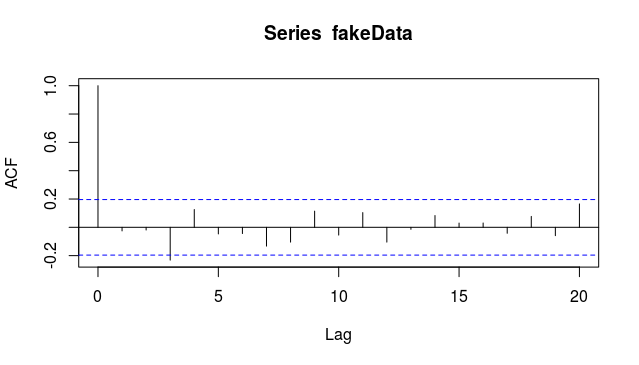
\includegraphics[width=100mm]{/home/taylor/UVa/all_teaching/4170_slides/2/2.5/pics/Rplot01.png}

\end{frame}


%----------------------------------------------------------------------------------------

\begin{frame}
\frametitle{When $h=1$: the one-step-ahead predictions}

% First, let's go back to some things we skipped in chapter 2.5.
% \newline

Now let's deal with $h=1$. Which means $X_{n+1}$ is predicted based on $X_1,\ldots,X_n$:
\[
X_{n+1} = \phi_{n1}X_n + \phi_{n2}X_{n-1} + \cdots + \phi_{nn} X_1 
\]
where
\[
\bm{\phi}_n = \Gamma_n^{-1}\bm{\gamma}_n
\]
where $\bm{\gamma}_n = (\gamma(1), \ldots, \gamma(n))'$ and $\bm{\phi}_n = (\phi_{n1},\ldots,\phi_{nn})'$.
\newline

We are inverting successively larger and larger matrices! That's very bad.
\newline

The Durbin-Levinson algorithm gives us $\bm{\phi}_{n}$ in terms of $\bm{\phi}_{n-1}$.
\end{frame}

%----------------------------------------------------------------------------------------

\begin{frame}
\frametitle{The Durbin-Levinson Algorithm}

\begin{block}{Durbin-Levinson}
$\bm{\phi}_{n}$ is computed recursively with the following:
\[
\phi_{nn} = \left[\gamma(n) - \sum_{j=1}^{n-1}\phi_{n-1,j}\gamma(n-j) \right] v_{n-1}^{-1}
\]
\[
\left[ \begin{array}{c}
\phi_{n,1} \\
\phi_{n,2} \\
\vdots \\
\phi_{n,n-1}
\end{array}\right]
=
\left[ \begin{array}{c}
\phi_{n-1,1} \\
\phi_{n-1,2} \\
\vdots \\
\phi_{n-1,n-1}
\end{array}\right]
- \phi_{n,n}
\left[ \begin{array}{c}
\phi_{n-1,n-1} \\
\phi_{n-1,n-2} \\
\vdots \\
\phi_{n-1,1}
\end{array}\right]
\]
and
\[
v_n = v_{n-1}[1 - \phi_{nn}^2]
\]
The initial points are $\phi_{11} = \rho(1)$ and $v_0 = \gamma(0)$.

\end{block}
\end{frame}


%----------------------------------------------------------------------------------------

\begin{frame}
\frametitle{The Durbin-Levinson Algorithm}

Inductive proof: divide both sides of $ \Gamma_n \bm{\phi}_n = \bm{\gamma}_n$ by $\gamma(0)$ to get
\[
\mathbf{R}_n \bm{\phi}_n = \bm{\rho}_n.
\]
Clearly this is satisfied for $n=1$. Suppose it is true for $n=k$ and show that the recursions from the last slide  imply that it's true for $n=k+1$. Let $\bm{\rho}_k^{(r)} = (\rho(k),\ldots,\rho(1))'$ and $\phi_k^{(r)} = (\phi_{kk},\ldots,\phi_{k1} )'$ (``r" stands for reverse).
\begin{align*}
\mathbf{R}_{k+1} \bm{\phi}_{k+1} &= 
\left[ \begin{array}{cc}
\mathbf{R}_k & \bm{\rho}_k^{(r)} \\
\bm{\rho}^{(r)'}_k   & 1
\end{array}\right]
\left[ \begin{array}{c}
\bm{\phi_k} - \phi_{k+1,k+1} \bm{\phi}_k^{(r)} \\
\phi_{k+1,k+1}
\end{array}\right] \\
&= 
\left[ \begin{array}{c}
\bm{\rho}_k - \phi_{k+1,k+1}\bm{\rho}_k^{(r)} + \phi_{k+1,k+1}\bm{\rho}_k^{(r)} \\
\bm{\rho}_k^{(r)'}\bm{\phi_k} - \phi_{k+1,k+1}\bm{\rho}_k^{(r)'}\bm{\phi}_k^{(r)} + \phi_{k+1,k+1}
\end{array}\right] \\
&= \bm{\rho}_{k+1}
\end{align*}
because $\mathbf{R}_k \bm{\phi}_k^{(r)} = \bm{\rho}_k^{(r)}$ too! Last line is a good homework question.
\end{frame}

%----------------------------------------------------------------------------------------

\begin{frame}
\frametitle{The Durbin-Levinson Algorithm}

Note done yet. Need to show the recursions for the mean square errors $v_n = E[(X_{n+1} - P_nX_{n+1})^2] $. Recall we had the initial condition $v_0 = \gamma(0)$, which is true because $P_0X_1 = E[X_1] = 0$. 
\begin{align*}
v_n &= \gamma(0) - \bm{\phi}_n'\bm{\gamma}_n \tag{2.5 slide 7} \\
&= \gamma(0) - 
\left[ \begin{array}{c}
\bm{\phi}_{n-1} -\phi_{nn}\phi_{n-1}^{(r)} \\
\phi_{nn}
\end{array}\right]' 
\left[\begin{array}{c}
\bm{\gamma}_{n-1} \\
\gamma(n)
\end{array}\right]\tag{DL2} \\
&= \gamma(0) - \phi_{n-1}'\gamma_{n-1} + \phi_{nn}\phi_{n-1}^{(r)'}\gamma_{n-1} - \phi_{nn}\gamma(n) \\
&= v_{n-1}+ \phi_{nn}\left( \phi_{n-1}^{(r)'}\gamma_{n-1} - \gamma(n) \right) \tag{2.5 slide 7} \\
&= v_{n-1} + \phi_{nn}\left( \gamma_{n-1}^{(r)'} \phi_{n-1} - \gamma(n) \right) \tag{algebra} \\
&= v_{n-1} - \phi_{nn}^2\left( \gamma(0) - \phi_{n-1}'\gamma_{n-1} \right) \tag{DL1} \\
&=v_{n-1}[1-\phi_{nn}^2]
\end{align*}

\end{frame}


%----------------------------------------------------------------------------------------

\begin{frame}
\frametitle{The Innovations Algorithm}

Suppose here that $X_t$ is a zero-mean time series with $E|X_t| < \infty$ for each $t$, and call $\kappa(i,j) = E[X_iX_j]$. Also denote the $1$-step ahead linear predictors as $\hat{X}_n = P_{n-1}X_n$ if $n > 1$ and $0$ if $n=1$. And denote their MSEs as $v_n = E(X_{n+1} - \hat{X}_{n+1})^2$.
\newline

The {\bf innovations} are 
\[
U_n = X_n - \hat{X}_n.
\]


\end{frame}

%----------------------------------------------------------------------------------------

\begin{frame}
\frametitle{The Innovations Algorithm}
$U_n = X_n - \hat{X}_n$ means that

\[
\left[ \begin{array}{c}
U_1 \\
U_2 \\
\vdots \\
U_n
\end{array}\right]
=
\left[ \begin{array}{ccccc}
1 & 0 & 0 & \cdots & 0 \\
a_{11} & 1 & 0 & \cdots & 0 \\
a_{22} & a_{2,1} & 1 & \cdots & 0 \\
\vdots & \vdots & \vdots & \ddots & 0 \\
a_{n-1,n-1} & a_{n-1,n-2} & a_{n-1,n-3} & \cdots & 1
\end{array}\right]
\left[\begin{array}{c}
X_1 \\
X_2 \\
\vdots \\
X_n
\end{array}\right]
\]
or in other words $\mathbf{U} = A_n \mathbf{X}_n$. We also know that $A_n^{-1} = C_n$ is lower-diagonal as well.

\end{frame}

%----------------------------------------------------------------------------------------

\begin{frame}
\frametitle{The Innovations Algorithm}

Our goal here is to write our predictions in terms of our errors.
\begin{enumerate}
\item $\mathbf{U}_n = \mathbf{X}_n - \hat{\mathbf{X}}_n$
\item $\mathbf{U}_n = A_n \mathbf{X}_n$
\item $C_n \mathbf{U}_n = \mathbf{X}_n$
\end{enumerate}
so
\begin{align*}
\hat{\mathbf{X}}_n &= \mathbf{X}_n - \mathbf{U}_n \\
&= C_n \mathbf{U}_n - \mathbf{U}_n \\
&= [C_n - I_n]\mathbf{U}_n \\
&= \Theta \mathbf{U}_n
\end{align*}

\end{frame}


%----------------------------------------------------------------------------------------

\begin{frame}
\frametitle{The Innovations Algorithm}

From the last slide we had $\hat{\mathbf{X}}_n = \Theta \mathbf{U}_n $ where
\[
\Theta = 
\left[ \begin{array}{ccccc}
0 & 0 & 0 & \cdots & 0 \\
\theta_{11} & 0 & 0 & \cdots & 0 \\
\theta_{22} & \theta_{21} & 0 & \cdots & 0 \\
\vdots & \vdots & \vdots & \ddots & 0\\
\theta_{n-1,n-1} & \theta_{n-1,n-2} & \theta_{n-1,n-3} & \cdots & 0
\end{array}\right]
\]
can be re-written as 
\[
\hat{X}_{n+1} = \sum_{j=1}^n\theta_{n,j}(X_{n+1-j} - \hat{X}_{n+1-j})
\]
if $n > 0$ and $\hat{X}_1 = 0$. Now we just need recursive formulas for these coefficients
\end{frame}

%----------------------------------------------------------------------------------------

\begin{frame}
\frametitle{Statement of Algorithm}

\begin{block}{The Innovations Algorithm}
The coefficients $\theta_{n1},\ldots,\theta_{nn}$ can be computed recursively from the equations
\[
v_0 = \kappa(1,1)
\]
\[
\theta_{n,n-k} = v_k^{-1}\left(\kappa(n+1,k+1) - \sum_{j=0}^{k-1}\theta_{k,k-j}\theta_{n,n-j} v_j \right),  \hspace{10mm} 0 \le k < n
\]
\[
v_n = \kappa(n+1,n+1) - \sum_{j=0}^{n-1}\theta_{n,n-j}^2v_j
\]
\end{block}

No proof given. 
\end{frame}


%----------------------------------------------------------------------------------------

\begin{frame}
\frametitle{Statement of Algorithm}

It goes...
\begin{enumerate}
\item $v_0$
\item $\theta_{11},v_1$
\item $\theta_{22},\theta_{21},v_2$
\item $\theta_{33},\theta_{32},\theta_{31}, v_3$
\item ...and so on...
\end{enumerate}
\end{frame}
%----------------------------------------------------------------------------------------

\begin{frame}
\frametitle{Throwback: Example 2.5.5}

Derive the recursive predictions for an ARMA(0,1) model
\[
X_t = Z_t + \theta_1 Z_{t-1}
\]
Everything besides diagonals and off-diagonals of $\kappa$ are $0$. 
\begin{enumerate}
\item $\kappa(i,i) = \gamma(0) = \sigma^2(1 + \theta^2)$
\item $\kappa(i,i+1) = \theta \sigma^2$
\end{enumerate}

Work on board:
\begin{enumerate}
\item $v_0 = (1+\theta^2)\sigma^2$
\item $v_n = (1 + \theta^2 - v_{n-1}^{-1}\theta^2\sigma^2)\sigma^2$
\item $\theta_{n1} = v_{n-1}^{-1}\theta\sigma^2$
\item and all other coefficients are $0$!
\end{enumerate}

\end{frame}


%----------------------------------------------------------------------------------------

\begin{frame}
\frametitle{Rule of Thumb}

General rule of thumb: use Innovations Algo for MA processes. Use Durbin-Levinson for AR processes.
\newline

For ARMA processes, we do something a little more clever. For ARMA processes where $p,q \ge 1$, section 3.3 describes how to use the innovations algorithm on a transformed series.
\end{frame}

\end{document} 